\documentclass[aspectratio=169,10pt]{beamer}

\usetheme{CambridgeUS}
\usecolortheme{beaver}
\usefonttheme{professionalfonts}

\usepackage[T1]{fontenc}
\usepackage[utf8]{inputenc}
\usepackage{lmodern}
\usepackage{amsmath,amssymb,booktabs,graphicx,array,tabularx}
\usepackage{makecell}

\definecolor{jhublue}{HTML}{002D72}
\definecolor{deepred}{HTML}{8A1538}
\definecolor{softgray}{HTML}{F3F5F7}

\setbeamercolor{structure}{fg=deepred}
\setbeamercolor{frametitle}{fg=white,bg=deepred}
\setbeamercolor{title}{fg=jhublue}
\setbeamercolor{block title}{fg=white,bg=jhublue}
\setbeamercolor{block body}{bg=softgray}
\setbeamertemplate{navigation symbols}{}
\setbeamertemplate{footline}[frame number]

\graphicspath{{figures/}}

\newcommand{\PPI}{\mathrm{PPI}}
\newcommand{\PPIPP}{\texttt{PPI++}}
\newcommand{\E}{\mathbb{E}}
\newcommand{\Var}{\mathrm{Var}}
\newcommand{\Cov}{\mathrm{Cov}}
\newcommand{\Corr}{\mathrm{Corr}}

\title[Prediction-Powered Inference and PPI]{Topics in Prediction-Powered Inference and Protein--Protein Interaction}
\author{Moran Guo}
\institute{ScM in Biostatistics\\Johns Hopkins Bloomberg School of Public Health}
\date{May 2026}

\begin{document}

\begin{frame}
  \titlepage
  \vspace{-0.35cm}
  \begin{center}
  \small Thesis advisor: Dr. Yiqun Chen \qquad Secondary reader: Dr. Ingo Ruczinski

  \vspace{0.25cm}
  
\includegraphics[width=0.42\textwidth]{BSPH.logo.cmyk_horizontal.blue.jpg}
  \end{center}
\end{frame}

\begin{frame}{Thesis Question}
\small
\begin{block}{Central problem}
Cheap model predictions can be generated for many units, while gold-standard (GS) labels are expensive and observed only on a smaller subset.
\end{block}

\vspace{-0.05cm}
\begin{block}{PPI/\texttt{PPI++} idea}
Do not treat ML predictions as truth. Instead, use predictions to cover many units and use a smaller GS subset to correct systematic prediction error.
\end{block}

\vspace{-0.05cm}
\begin{columns}[T,totalwidth=\textwidth]
\begin{column}{0.49\textwidth}
\textbf{PPI}
\begin{itemize}
  \item Combines broad predictions with scarce labels.
  \item Corrects estimates using labeled residual error.
\end{itemize}
\end{column}
\begin{column}{0.49\textwidth}
\texttt{PPI++}
\begin{itemize}
  \item Adds data-adaptive weight parameter.
  \item Trusts predictions more only when they help.
\end{itemize}
\end{column}
\end{columns}

\vspace{0.15cm}
\textbf{Thesis question:} when can this strategy support reliable estimation, uncertainty quantification, and study planning for protein-interaction questions?
\end{frame}

\begin{frame}{Logic of the Talk}
\begin{block}{Flow}
Start with the intuition, introduce notation only after the problem is clear, then use that notation to connect methodology to the protein application.
\end{block}

\begin{enumerate}
  \item \textbf{Setup and notation.} Define labels, predictions, calibration data, and target quantities.
  \item \textbf{Foundation I: after labels are observed.} How can noisy or biased surrogate labels be corrected efficiently?
  \item \textbf{Foundation II: before labels are collected.} How does surrogate quality change power and labeled-sample planning?
  \item \textbf{Protein application.} Build a leakage-aware protein-edge surrogate, freeze it, then use it for corrected estimation and planning.
\end{enumerate}

\vspace{0.15cm}
\begin{block}{Takeaway}
The prediction model is only the first layer. The statistical layer asks whether those predictions can support calibrated estimates, uncertainty intervals, and label-budget decisions.
\end{block}
\end{frame}

\begin{frame}{Statistical Notation}
\small
\begin{tabularx}{\textwidth}{@{}lX@{}}
\toprule
Symbol & Meaning in the thesis \\
\midrule
\(i\) or \(e=(u,v)\) & Generic unit (one observation); a protein-pair edge in the protein application. \\
\(X_i\) & Raw inputs or features used to produce a surrogate prediction. \\
\(Y_i\) & Gold-standard (GS) outcome; for binary edges, whether the edge is labeled positive. \\
\(f_i=f(X_i)\) or \(\hat p_e\) & Cheap surrogate prediction. \\
\(R_i\) & Indicator that the GS label is observed or not. \\
\(L=\{i:R_i=1\}\), \(n=|L|\) & Labeled calibration or pilot sample. \\
\(U=\{i:R_i=0\}\), \(N=|U|\) & Prediction-only sample with surrogate labels but no GS labels. \\
\(\theta=\E(Y_i)\) & Primary mean estimand; for binary edges, a prevalence or positive-edge rate. \\
\(\lambda\) & \PPIPP{} tuning weight controlling how strongly predictions contribute to the estimator. \\
\(\rho^2_{Y,f}\) & Squared truth-surrogate correlation; the key pilot quantity for planning. \\
\(\Delta\) & Target absolute difference in a mean/proportion-type estimand (power analysis). \\
\bottomrule
\end{tabularx}
\end{frame}

\begin{frame}{Prediction-Powered Estimator Family}
\textbf{Original PPI mean estimator}
\[
\widehat{\theta}_{\PPI}
=
\overline{f}_{U}
+
\frac{1}{n}\sum_{i\in L}(Y_i-f_i)
\]

\textbf{Tuned \PPIPP{} estimator}
\[
\widehat{\theta}_{\lambda}
=
\overline{Y}_{L}
+
\lambda(\overline{f}_{U}-\overline{f}_{L})
\]

\begin{columns}[T,totalwidth=\textwidth]
\begin{column}{0.49\textwidth}
\begin{block}{Correction logic}
\begin{itemize}
  \item Use predictions at scale for broad coverage.
  \item Use labels on \(L\) to estimate residual error.
  \item Target remains the GS label estimand.
\end{itemize}
\end{block}
\end{column}
\begin{column}{0.49\textwidth}
\begin{block}{Tuning logic}
\begin{itemize}
  \item \(\lambda=1\): vanilla PPI.
  \item \(\hat\lambda\): estimated from pilot data.
  \item Weak surrogates should receive limited weight.
\end{itemize}
\end{block}
\end{column}
\end{columns}
\end{frame}

\begin{frame}{Foundation I-A: Noisy Surrogates}
\textbf{Motivating example:} LLM-as-a-judge evaluation, where human preference labels are scarce and cheaper judge labels are noisy.

\vspace{0.15cm}
\begin{columns}[T,totalwidth=\textwidth]
\begin{column}{0.49\textwidth}
\begin{block}{Classical view}
\begin{itemize}
  \item Cheap label is an imperfect diagnostic measurement.
  \item Bias can be corrected with sensitivity/specificity-style quantities.
  \item Rogan--Gladen is the binary reference case.
\end{itemize}
\end{block}
\end{column}
\begin{column}{0.49\textwidth}
\begin{block}{Prediction-powered view}
\begin{itemize}
  \item Cheap signal is a generic surrogate.
  \item Calibration set estimates residual error.
  \item Flexible enough for continuous model scores.
\end{itemize}
\end{block}
\end{column}
\end{columns}

\vspace*{0.2cm}
\textbf{Relevance:} the protein surrogate is not a human judge label, but the missing-label structure is the same: \(Y\) is expensive, \(f(X)\) is cheap, and calibration is essential.
\end{frame}

\begin{frame}{Foundation I-B: Efficient Correction}
Let \(\mu(\widehat Y)=\E(Y\mid \widehat Y)\), \(R\) indicate observed GS labels, and \(\pi=\Pr(R=1)\).

\textbf{Efficient influence function for \(\theta=\E(Y)\)}
\[
\phi(O)
=
\mu(\widehat{Y})-\theta
+
\frac{R}{\pi}\{Y-\mu(\widehat{Y})\}.
\]

\textbf{Corresponding residual-correction estimator}
\[
\widehat{\theta}(\mu)
=
\frac{1}{N}\sum_{i\in U}\mu(\widehat{Y}_i)
+
\frac{1}{n}\sum_{i\in L}\{Y_i-\mu(\widehat{Y}_i)\}.
\]

\begin{block}{Main statistical takeaway}
Better surrogates help twice: they improve prediction, and they reduce residual variation after calibration, which can shorten uncertainty intervals for the target estimand.
\end{block}
\end{frame}

\begin{frame}{Foundation II-A: Variance and \(\lambda\)}
For the \PPIPP{} mean estimator,
\[
\Var(\widehat{\theta}_{\lambda})
=
\frac{\Var(Y-\lambda f)}{n}
+
\frac{\lambda^2\Var(f)}{N}.
\]

Expanding the first term shows the bias-variance tradeoff:
\[
\Var(\widehat{\theta}_{\lambda})
=
\frac{\Var(Y)}{n}
+
\lambda^2\Var(f)\left(\frac{1}{n}+\frac{1}{N}\right)
-
\frac{2\lambda\Cov(Y,f)}{n}.
\]

The oracle tuning value is
\[
\lambda^\star
=
\frac{\Cov(Y,f)}
{\Var(f)(1+n/N)}.
\]

\textbf{Interpretation:} strong covariance between \(Y\) and \(f\) justifies borrowing from the prediction-only sample; weak covariance makes aggressive borrowing inefficient.
\end{frame}

\begin{frame}{Foundation II-B: Planning}
Substituting \(\lambda^\star\) gives
\[
\Var(\widehat{\theta}_{\lambda^\star})
=
\frac{\Var(Y)}{n}
\left(1-\frac{\rho^2_{Y,f}}{1+n/N}\right),
\qquad
\rho_{Y,f}=\Corr(Y,f).
\]

For target difference \(\Delta\), two-sided level \(\alpha\), and power \(1-\beta\),
\[
S^2=
\left(\frac{\Delta}{z_{1-\alpha/2}+z_{1-\beta}}\right)^2,
\qquad
n_{\mathrm{req}}(\lambda)
=
\frac{\Var(Y-\lambda f)}
{S^2-\lambda^2\Var(f)/N}.
\]

\begin{block}{Design consequence}
When \(N\gg n\), labeled-sample savings are driven approximately by \(\rho^2_{Y,f}\). This is why the protein planning analysis focuses on pilot \(\rho^2_{Y,\hat p}\), not only PR-AUC or ROC-AUC.
\end{block}
\end{frame}

\begin{frame}{Protein Application: Data and Pipeline}
\begin{columns}[T,totalwidth=\textwidth]
\begin{column}{0.47\textwidth}
\textbf{Scientific target}
\begin{itemize}
  \item Positive edge: benchmark-defined physical protein--protein interaction.
  \item Intra: predefined positives and negatives.
  \item BIOGRID-human: curated physical positives and sampled non-positive negatives.
  \item Merged training pool: 896,858 leakage-controlled edges.
\end{itemize}

\vspace{0.15cm}
\small
\begin{center}
  \begin{tabular}{llr}
  \toprule
  Dataset & Split & Total\\
  \midrule
  Intra & Train & 163,192\\
  Intra & Val./pilot & 59,260\\
  Intra & Test & 52,048\\
  BIOGRID & Test & 36,769\\
  Merged & Train & 896,858\\
  \bottomrule
  \end{tabular}
  \end{center}
\end{column}
\begin{column}{0.51\textwidth}
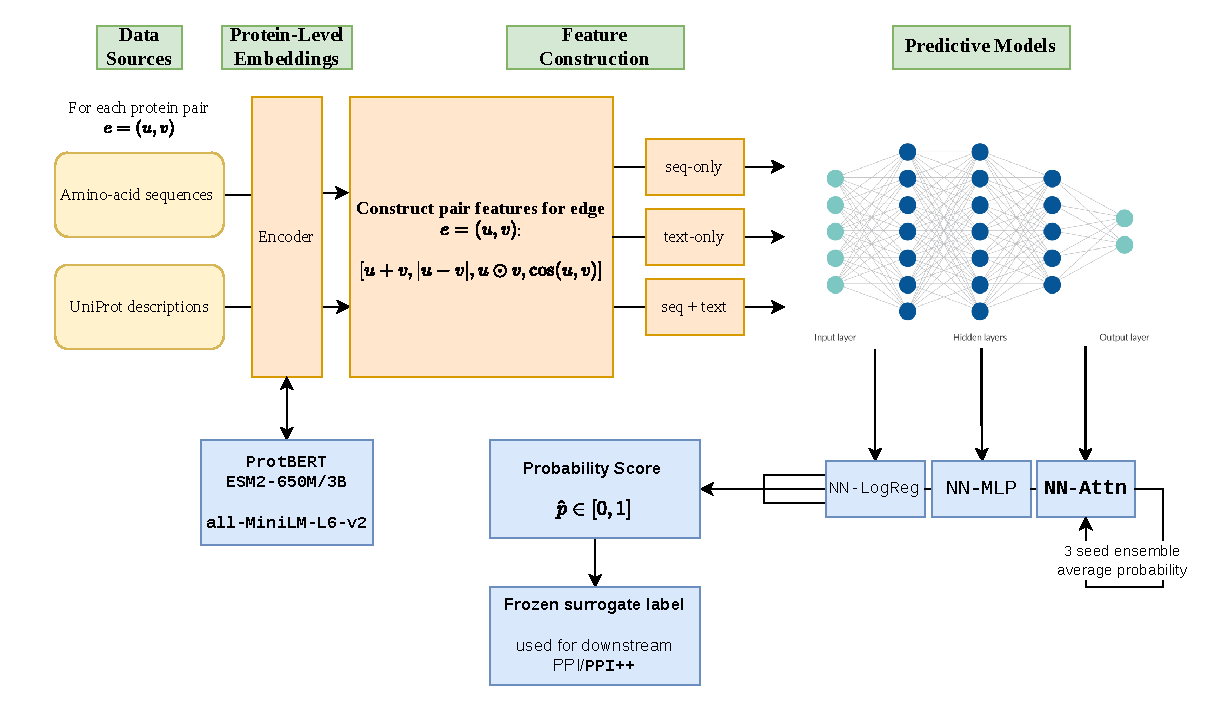
\includegraphics[width=\linewidth,height=0.63\textheight,keepaspectratio]{Pipeline_thesis.pdf}

\vspace{0.05cm}
\small
\textbf{Frozen surrogate:} sequence-plus-text ESM2-3B attention ensemble, averaged across three random seeds.
\end{column}
\end{columns}
\end{frame}

\begin{frame}{Protein Prediction Layer}
\begin{center}
\small
\begin{tabular}{lccccc}
\toprule
Model & \makecell{Intra val\\PR} & \makecell{Intra test\\PR} & \makecell{Intra test\\ROC} & \makecell{BIOGRID\\PR} & \makecell{BIOGRID\\ROC}\\
\midrule
Seq LogReg & 0.60 & 0.62 & 0.62 & 0.76 & 0.78\\
Seq MLP & 0.67 & 0.68 & 0.70 & 0.78 & 0.79\\
Seq+Text MLP & 0.68 & 0.70 & 0.71 & 0.78 & 0.80\\
Seq+Text Attn & 0.69 & 0.70 & 0.71 & 0.79 & 0.80\\
\textbf{Attn Ensemble} & \textbf{0.70} & \textbf{0.72} & \textbf{0.72} & \textbf{0.80} & 0.81\\
Log-loss Ens. & 0.64 & 0.65 & 0.67 & 0.80 & \textbf{0.82}\\
\bottomrule
\end{tabular}
\end{center}

\vspace{0.15cm}
\begin{itemize}
  \item The frozen attention ensemble is strongest on the main in-domain test split.
  \item The log-loss ensemble improves one external loss-oriented metric but weakens in-domain ranking and pilot \(\rho^2_{Y,\hat p}\).
  \item The chosen model is a stable inferential surrogate, not only a benchmark classifier.
\end{itemize}
\end{frame}

\begin{frame}{Protein Inference Layer}
\begin{block}{Prediction-to-inference handoff}
After model selection, seed-level probabilities are averaged into one fixed edge score \(\hat p_e\). PPI and \PPIPP{} then use calibration budgets of 5\%, 10\%, and 20\% of each held-out test split.
\end{block}

\vspace{0.1cm}
\begin{center}
\scriptsize
\begin{tabular}{lllccc}
\toprule
Dataset & Budget & Metric & Truth & PPI 95\% CI & \PPIPP{} 95\% CI\\
\midrule
Intra & 5\% & Prevalence & 0.50 & 0.50 [0.48, 0.51] & 0.50 [0.48, 0.51]\\
Intra & 5\% & Accuracy & 0.66 & 0.66 [0.64, 0.68] & 0.66 [0.64, 0.67]\\
Intra & 5\% & Brier & 0.34 & 0.34 [0.33, 0.36] & 0.34 [0.33, 0.36]\\
BIOGRID & 5\% & Prevalence & 0.48 & 0.48 [0.47, 0.50] & 0.48 [0.47, 0.50]\\
BIOGRID & 5\% & Accuracy & 0.71 & 0.71 [0.69, 0.73] & 0.71 [0.69, 0.73]\\
BIOGRID & 5\% & Brier & 0.29 & 0.29 [0.27, 0.31] & 0.29 [0.27, 0.31]\\
\bottomrule
\end{tabular}
\end{center}

\textbf{Interpretation:} corrected estimates remain close to full-data references even at the smallest reported calibration budget.
\end{frame}

\begin{frame}{Protein Planning Layer}
\begin{columns}[T,totalwidth=\textwidth]
\begin{column}{0.43\textwidth}
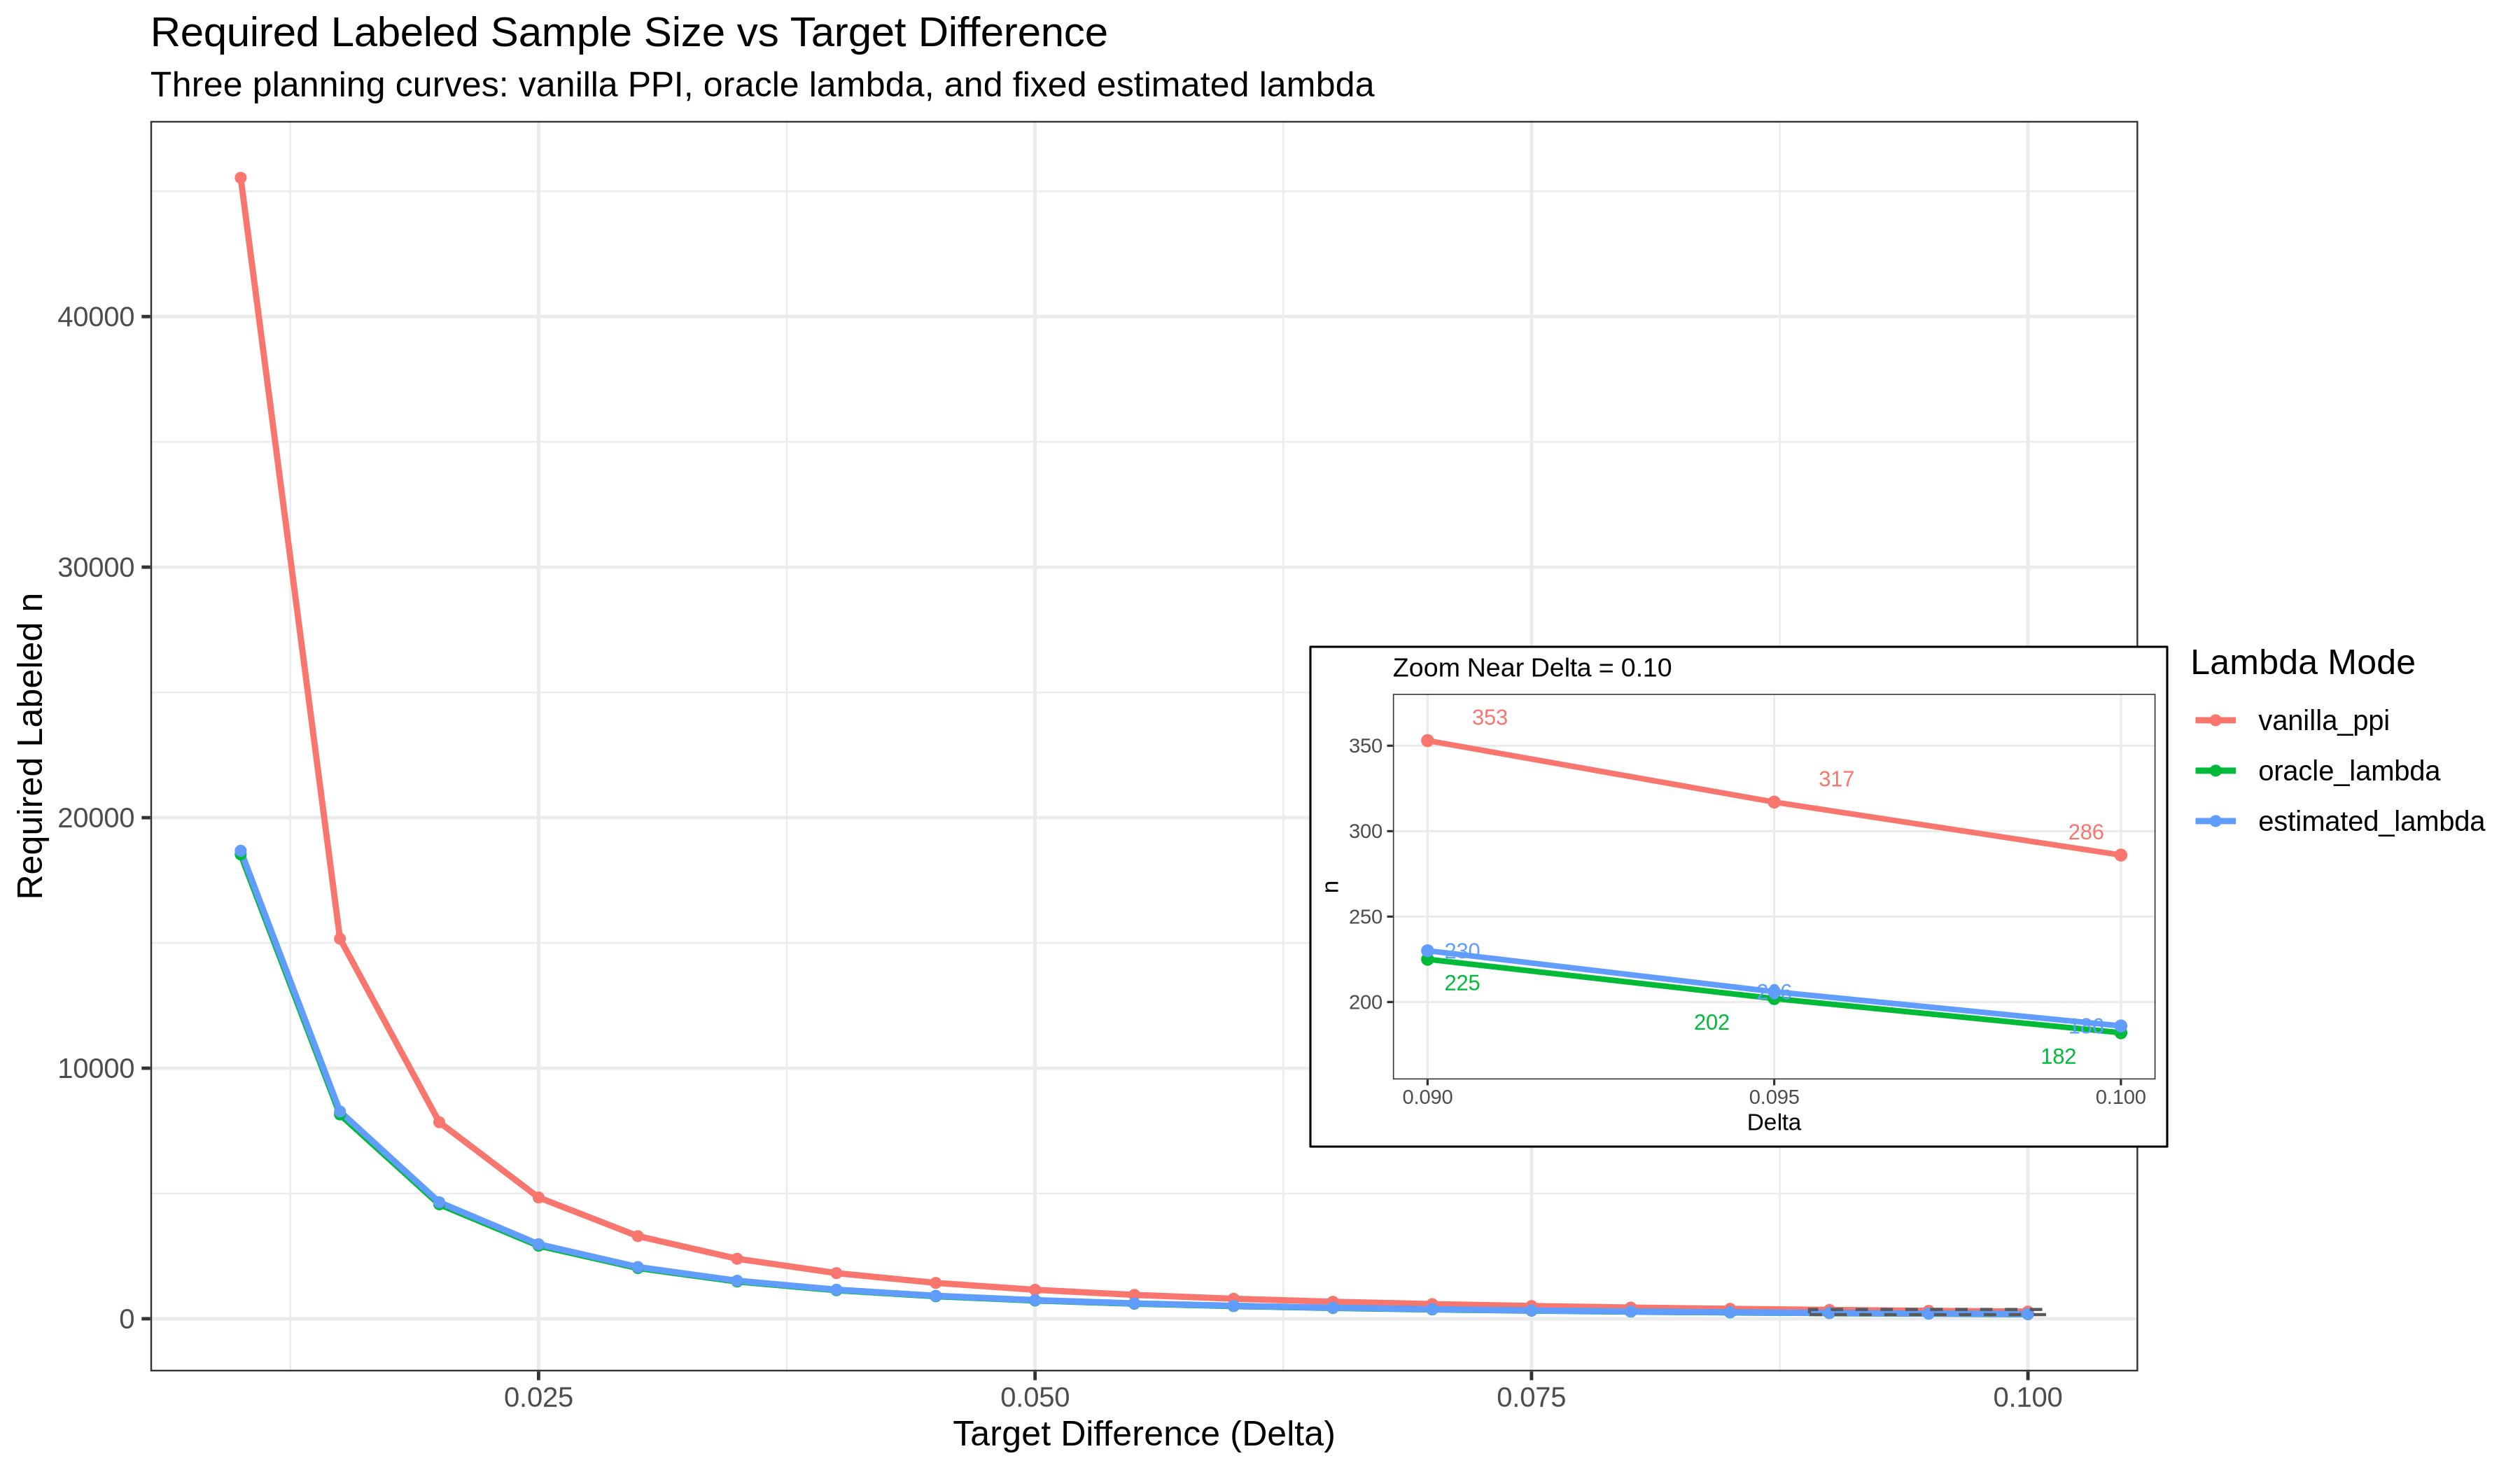
\includegraphics[width=\linewidth]{chap5_required_n_curves_zoom.png}
\end{column}
\begin{column}{0.55\textwidth}
\small
\textbf{Required labels for prevalence-like target}
\begin{center}
\begin{tabular}{lccc}
\toprule
Method & \(\Delta=.02\) & \(\Delta=.05\) & \(\Delta=.10\)\\
\midrule
Classical & 4906 & 785 & 197\\
Vanilla PPI & 7844 & 1155 & 286\\
Est. \PPIPP{} & 4649 & 743 & 186\\
Oracle \PPIPP{} & 4567 & 727 & 182\\
\bottomrule
\end{tabular}
\end{center}

\textbf{Surrogate-strength story}
\begin{itemize}
  \item Pilot \(\rho^2_{Y,\hat p}\) increases from 0.03 for Seq LogReg to 0.11 for the attention ensemble.
  \item At \(\Delta=0.05\), required labels fall from 785 classically to 726 for the ensemble.
  \item Gains are real but moderate because the protein surrogate is only moderately correlated with the GS labels.
\end{itemize}
\end{column}
\end{columns}
\end{frame}

\begin{frame}{Protein-Specific Interpretation}
\textbf{What the application shows}
\begin{itemize}
  \item Leakage-aware sequence-plus-text modeling can produce a usable protein-edge surrogate.
  \item PPI and \PPIPP{} correction are stable on both Intra and BIOGRID held-out splits.
  \item Tuned \PPIPP{} matters because vanilla PPI can over-borrow from a modest surrogate.
\end{itemize}

\vspace{0.15cm}
\textbf{Main limitation: published planning formulas are i.i.d.}
\begin{itemize}
  \item Protein-pair observations are graph-structured edges.
  \item Two observed edges can share an endpoint protein, creating dependence.
  \item The planning curves should be read as an i.i.d. baseline, not as dependence-robust guarantees.
\end{itemize}

\begin{block}{Next methodological step}
Develop prediction-powered variance estimators and sample-size formulas for graph-dependent edge observations.
\end{block}
\end{frame}

\begin{frame}{Main Findings}
\begin{enumerate}
  \item Prediction-powered inference gives a coherent workflow for scarce GS labels and broad cheap predictions.
  \item The noisy-surrogate foundation explains why residual correction can target the GS label estimand even when the surrogate is biased.
  \item The planning foundation shows that label savings are governed by pilot \(\rho^2_{Y,f}\).
  \item The protein attention ensemble is a useful but moderate-strength surrogate.
  \item Corrected protein estimates track full-data references under limited calibration budgets.
  \item Planning gains are present but modest, and dependence is the major unresolved issue.
\end{enumerate}
\end{frame}

\begin{frame}{Closing Message}
\begin{center}
\Large \textbf{Strong predictions help most when they are used as calibrated statistical surrogates, not as replacements for validation labels.}
\end{center}

\vspace{0.4cm}
\begin{columns}[T,totalwidth=\textwidth]
\begin{column}{0.49\textwidth}
\textbf{For biostatistics}
\begin{itemize}
  \item Separate prediction quality from inferential validity.
  \item Use labeled subsets to correct and quantify uncertainty.
  \item Treat planning assumptions explicitly.
\end{itemize}
\end{column}
\begin{column}{0.49\textwidth}
\textbf{For protein-interaction studies}
\begin{itemize}
  \item Leakage-aware benchmark construction is essential.
  \item Surrogate scores can support calibrated prevalence-like summaries.
  \item Graph dependence needs new theory before strong guarantees.
\end{itemize}
\end{column}
\end{columns}
\end{frame}

\end{document}
